% !TEX root = ../main.tex
% Chapter Experimental setup

\chapter{Experimental setup} % Main chapter title

\label{Chapter3} % Change X to a consecutive number; for referencing this chapter elsewhere, use \ref{ChapterX}

This chapter reviews the different experiments undertaken during this thesis. The goal of these experiments is to measure the effectiveness of more complex models against simple ones, different preprocessing strategies and the computational performance between different GPUs. All models are trained with the Cornell Movie Dialogs corpus.

\section{Cornell Movie Dialogs corpus}
The Cornell Movie Dialogs corpus \citep{cornell} is constructed from raw movie scripts. It has 220,579 conversational exchanges between 10,292 pairs of movie characters involving 9,035 characters from 617 movies. Here are some examples from the corpus.

\begin{center}
    ``You have my word.  As a gentleman'' - ``You're sweet.''\\
    ``There.'' - ``Where?''\\
    ``Gosh, if only we could find Kat a boyfriend...'' - ``Let me see what I can do.''
\end{center}

The texts have very different lengths. Table~\ref{tab:stats-cornell} shows some statistics of text lengths and Figure~\ref{fig:hist-cornell-senteces-length} illustrates the conversations' length distribution. The large majority of conversations does not exceed 15 words.

\begin{table}
    \centering
    \caption[Statistics sentence corpus length]{Statistics of sentences' lengths for Cornell Movie Dialogs corpus. All measures are letter-wise and not word-wise, except ``Utterances'' that simply represent the number of conversations in the dataset.}
    \label{tab:stats-cornell}
    \begin{tabular}{c|ccccccc}
        \toprule
        \tabhead{Utterances} & \tabhead{Mean} & \tabhead{Min} & \tabhead{Max} & \tabhead{Std} & \tabhead{25\%} & \tabhead{50\%} & \tabhead{75\%}\\
        \midrule
        304713 & 55.32 & 1 & 3046 & 64.09 & 19 & 35 & 69\\
        \bottomrule
    \end{tabular}
\end{table}

\begin{figure}
    \centering
    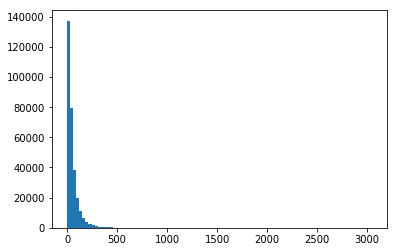
\includegraphics[width=.8\textwidth]{hist_cornell_sentences_length}
    \decoRule
    \caption[Conversations length distribution]{Conversations length distribution. The average word length in English is about five letters~\citep{wolframlanguage}, thus the large majority of the conversations does not exceed 15 words. X-axis represents the sentences lengths (letter-wised) and Y-axis represents the number of sentences.}
    \label{fig:hist-cornell-senteces-length}
\end{figure}

\section{Experiments model architecture}
The general purpose of this chatbot is to learn how to converse with other humans based on the movie dialogs. The model's architecture follows the Neural Machine Translation (NMT) model.
Instead of translating from a language to another, the model ``translates'' the question into an answer, since the input and output have the same form in both cases.

Since dialogs in movies are open-domain conversations, just splitting the dataset into an 80-10-10 division (80\% training set, 10\% development set, 10\% test set, \citet{jurafsky2014speech})to train models might not work well. Thus, the idea is to find a closer domain even in this context by trying to train the model to act like one the movie character. To ensure that the training does not suffer from the lack of data, the character is chosen based on the number of conversations he is involved into. Table~\ref{tab:char-cornell} shows the five most present characters.

\begin{table}
    \caption[Character presence analysis]{Character presence analysis within the Cornell Movie Dialogs corpus presenting the five most present character.}
    \label{tab:char-cornell}
    \centering
    \begin{tabular}{llllll}
        \toprule
        & \tabhead{Jack} & \tabhead{Joe} & \tabhead{George} & \tabhead{Frank} & \tabhead{Nick}\\
        \midrule
        \tabhead{Utterances} & 3032 & 1897 & 1748 & 1537 & 1484\\
        \bottomrule
    \end{tabular}
\end{table}

In all the different runs, the training is done in two phases, namely the training, based on all the conversations, and the fine-tuning, based only on the conversations where the chosen character is answering. Other features like the gender of the character speaking first might lead to better results.


\section{Infrastructures}
% Tensorflow is able to run on both CPU and GPU systems without changing the code. Thus, preparing the script on a local computer and performing the training on a server is easily feasible.
The server used in this thesis is hosted on a GPU accelerated cloud platform, Paperspace\footnote{https://www.paperspace.com/} with pre-configured flavors for machine learning applications. The machine used for all experiments is the ``\textit{GPU+}'' flavor configured with 30GB RAM, 8 CPU cores and a dedicated NVIDIA Quadro M4000. Only one training was performed also on another machine to analyze if the cost of a more expensive flavor is worth the time saved.
The more expensive is actually the most expensive one proposed by Paperspace with a dedicated last-generation NVIDIA Tesla V100, Volta generation. Table~\ref{tab:paperspace-flavors} summarizes the differences between the two flavors. The ``\textit{V100}'' flavor costs almost 6 times more than the other flavor.

\begin{table}
    \centering
    \caption[Paperspace flavors]{Paperspace dedicated GPU flavors differences.}
    \label{tab:paperspace-flavors}
    \begin{tabular}{lllllll}
        \toprule
        \tabhead{Flavor} & \tabhead{Generation} & \tabhead{VRAM} & \tabhead{Bandwith} & \tabhead{Performance} & \tabhead{Price}\\
        \midrule
        GPU+ & Maxwell & 8 GB & 192 GB/s & 2.6 teraFLOPS & \$0.40 per hour\\
        V100 & Volta & 16 GB & 900 GB/s & 112 teraFLOPS & \$2.30 per hour\\
        \bottomrule
    \end{tabular}
\end{table}
